
% ==========================================================

\chapter{Генерация и транспорт убегающих электронов в плазме токамаков, а так же использование сцинтиляционных детекторов для их диагностики}
\label{ch:ch1}

% ==========================================================

\section{Механизмы генерации убегающих электронов}\label{sec:ch1/sec1}

В плазме токамаков имеют место несколько механизмов генерации убегающих электронов. Это:

\begin{itemize}
  \item <<традиционный>> механизм генерации убегающих электронов в электрическом поле;
  \item лавинный механизм, при котором первичные убегающие электроны при взаимодействии с электронами основной плазмы перевозят их в режим убегания;
  \item прочие механизмы, такие как генерация убегающих электронов при распаде трития или при комптоновском рассеянии гамма излучения.
\end{itemize}

Рассмотрим ниже эти механизмы подробнее.

% ----------------------------------------------------------

\subsection{Убегание электронов в сильных электрических полях в плазме}

Эффект убегания был предсказан в 1925 году \cite{Wilson1925} и развит в \cite{Dreicer1959}. Пусть в сильноионизованной плазме имеется электрическое поле $E$. Тогда для перехода в режим непрерывного ускорения сила, действующая на электрон со стороны электрического поля, должна превышать силу трения, вызванную кулоновскими столкновениями в плазме:

\begin{equation}
  \label{eq:runawayEq}
  e E >  m_e v_e \nu_{ei}(v_e)
\end{equation}
где $e$ и $m_e$ --- заряд и масса электрона, $\nu_{e}$ --- частота столкновений электрона, $v$ --- скорость электрона \cite{Wesson2004}. Частота кулоновских электрон-ионных столкновений зависит от скорости. Для случая, когда $v \gg \sqrt{ 2 T_e / m_e }$, где $T_e$ --- средняя температура электронов, частота электронных столкновений может быть представлена как 
\begin{equation*}
  \nu_{e}(v) = \frac{ 3 e^4 n \Lambda }{ 4 \pi \epsilon_0^2 m_e^2 v^3 }
\end{equation*} 
где $\Lambda$ --- кулоновский логарифм, $n$ --- концентрация плазмы \cite{Wesson2004}. Графики зависимости силы, действующей на электрон со стороны электрического поля, и силы трения, показаны на рисунке~\ref{fig:runawayForces}.

\begin{figure}[ht]
  \centerfloat{ 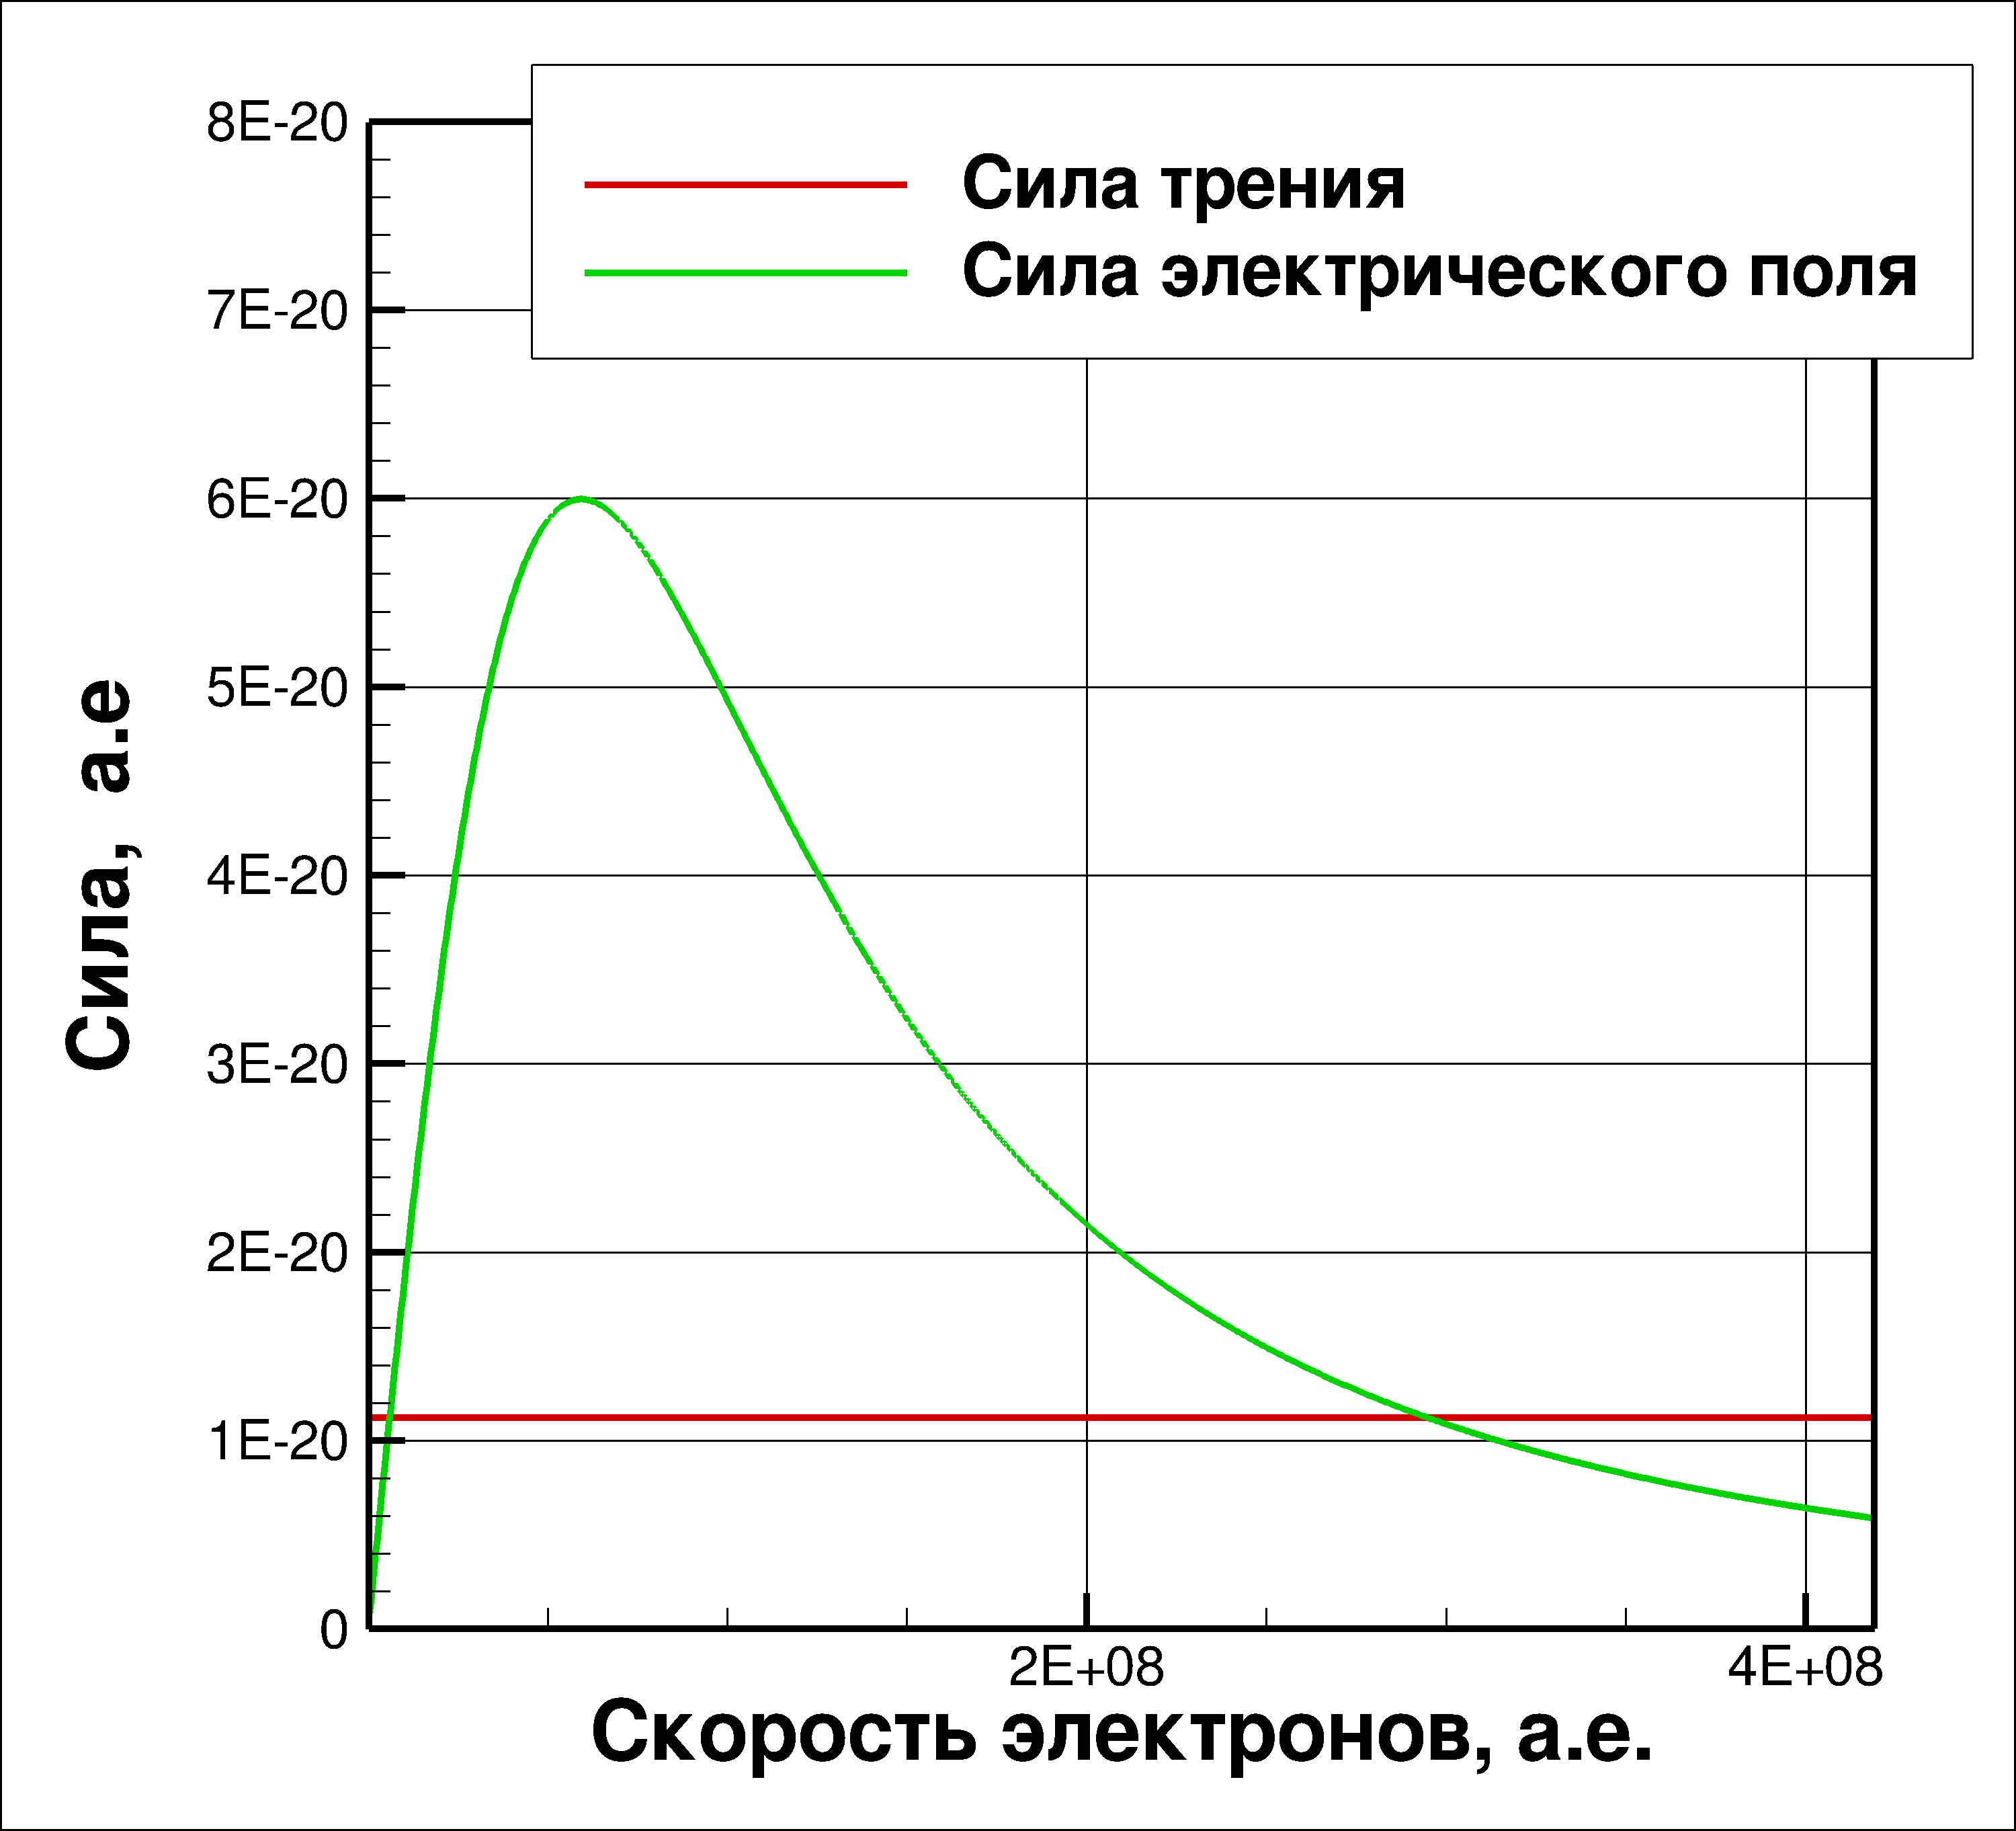
\includegraphics[width=0.60\linewidth]{runawayForces} }
  \caption{ Зависимотсть силы, действующей на электрон со стороны электрического поля и силы трения, которая вычислена по формуле $ C \cdot v/( v^2 + v_{Te}^2 )^{3/2} $~\cite{Golant1977}.}
  \label{fig:runawayForces}
\end{figure}

Можно заметить, что существует некая критическая скорость, начиная с которой неравенство \ref{eq:runawayEq} оказывается истинным. Эта критическая скорость равна
\begin{equation}
  \label{eq:critVelocity}
  v_c = \sqrt{ \frac{ 3 e^3 n \Lambda }{ 4 \pi \epsilon_0^2 m_e E } }
\end{equation}
Если каким-то образом образуется электрон со скоростью, больше критической скорости $v_c$, то он переходит в режим неограниченного ускорения. Такие электроны называются <<убегающими>> \cite{Golant1977}.

Можно рассчитать величину электрического поля, при котором в режим убегания переходят электроны с тепловой скоростью. Это поле оказывается равным 
\begin{equation*}
  E_D = \frac{ n e^3 \Lambda }{ 4 \pi \epsilon_0^2 m_e v_{Te}^2 }
\end{equation*}
и называется полем Дрейсера \cite{Dreicer1959,Golant1977,Wesson2004}. 

Когда электрическое поле достаточно мало, критическая скорость, рассчитанная по уравнению \ref{eq:critVelocity}, приближается к скорости света $c$. Для релятивистских электронов время замедления почти постоянно и существенного уменьшения силы трения с увеличением их энергии уже не происходит. Соответственно, для электрических полей, таких что
\begin{equation*}
  E < E_c = \frac{ n e^3 \Lambda }{ 4 \pi \epsilon_0^2 m_e c^2 }
\end{equation*}
генерации убегающих электронов не происходит ни при каких обстоятельствах \cite{Wesson2004}.

На большем временном масштабе скорость убегания электронов определяется столкновительной диффузией в пространстве скоростей. По мере убегания более быстрых электронов они замещаются электронами, диффундирующими через хвост максвелловского распределения скоростей. Подробные расчеты дают следующую результирующую скорость убегания на единицу объема \cite{Wesson2004}: 
\begin{equation*}
  S_{re} = \frac{2}{ \sqrt{\pi} } n \nu_{e}(v_{Te}) \left( \frac{E}{E_D} \right)^{1/2} \exp\left( -\frac{E_D}{4 E} - \left( \frac{2 E_D }{E} \right)^{1/2} \right)
\end{equation*}


% ----------------------------------------------------------

\subsection{Лавинный эффект размножения убегающих электронов}

При кулоновских столкновениях между <<быстрыми>> убегающими электронами и <<медленными>> электронами основной плазмы первые могут передавать вторым часть своей энергией, переводя их в режим убегания \cite{Sokolov1979}. Очевидно, для работы этого процесса требуется, чтобы время жизни убегающего электрона было больше времени между кулоновскими столкновениями. Темп генерации оказывается пропорциональным числу уже существующих в плазме убегающих электронов \cite{Rozansky2012}.  Хотя на пробные частицы в плазме в основном влияют столкновения с большими прицельными параметрами и малым переданным импульсом, в этом процессе большее значение имеет меньшее число близких столкновений, передающих больший импульс. Соответствующие близкие столкновения в этом случае --- это те, которые поднимают медленный электрон выше критической скорости для убегания. 

Импульс, передаваемый медленному электрону быстрым электроном, в основном перпендикулярен скорости $v_f$ быстрого электрона и определяется выражением
\begin{equation*}
  m_e \Delta v \approx 2 m_e v_f \frac{r_0}{r}
\end{equation*}
где $r$ --- прицельный параметр, а $r_0 = e^2 / 4 \pi \epsilon_0 m_e v_f^2$ --- значение прицельного параметра для рассеяния на 90$^\circ$ \cite{Wesson2004}. 

Чтобы столкновение перенесло электрон в область убегания, $\Delta v$ должна быть больше критической скорости, определяемой уравнением \ref{eq:critVelocity}. С учётом этого требования, можно написать сечение для рождения убегающего электрона:
\begin{equation*}
  \sigma(v_f) = \frac{ e E }{ 3 n m_e v_f^2 \Lambda }
\end{equation*}
Считая убегающие электроны релятивистскими, можно положить что $v_f = c$. Тогда скорость рождения новых убегающих электронов оказывается равна следующей величине \cite{Rozansky2012}:
\begin{equation}
  \label{eq:avalanch}
  \frac{ d n_r }{ d t } = n_r \nu_e(c) \left( \frac{E}{E_c} - 1 \right) / \left( 2 \Lambda \right)
\end{equation}
Множитель $E/E_c - 1 $ в формуле \ref{eq:avalanch} показывает, что лавинный механизм генерации убегающих электронов имеет пороговый характер.

Подробно теория генерации убегающих электронов изложена в \cite{Rosenbluth1997}. Лавинный механизм генерации убегающих электронов неоднократно наблюдался в экспериментах; впервые оно было экспериментально обнаружено на токамаке TEXTOR, вероятно имеет место во время срывов на токамаках TFTR, Tore Supra, JT-60U и JET \cite{Gill2002,Helander2002}, было зарегистрировано на токамаке TCABR \cite{Galvao2001}. Анализ распределения по энергии убегающих электронов позволяет предположить, что лавинный механизм может быть доминирующим при генерации убегающих электронов во время срывов, а в срывах JET кажется трудным объяснить ток, переносимый убегающими электронами, не прибегая к этому механизму \cite{Helander2002}.


% ----------------------------------------------------------

\subsection{Прочие механизмы генерации убегающих электронов}

Прочие механизмы генерации убегающих электронов носят скорее экзотический характер и не являются существенными на современных установках, однако могут оказывать влияние на более крупных токамаках будущего. Эти механизмы могут служить источником первичных убегающих электронов, которые могут потом размножаться по лавинному механизму за счёт кулоновских столкновений.

При радиоактивном распаде трития, который будет являться одним из компонентов топливной смеси промышленных термоядерных установок, образуется электрон \cite{Burrows1990}:
\begin{equation*}
  T \rightarrow {}^3_2 He + e^{-} + \bar{ \nu_e }
\end{equation*}
Период полураспада трития составляет $ \tau_T = 4500 $ дней, максимальная энергия рождённых в ходе распада электронов равна $ E_{max} = 18.6$~кэВ \cite{MartinSolis2017}. Число убегающих электронов, рождённых за счёт подобного механизма, составляет

\begin{equation*}
  \left( \frac{ d n_{re} }{ d t } \right) \approx \ln(2) \frac{ n_T }{ \tau_T } F_{\beta}(\varepsilon_c)
\end{equation*}
где $\varepsilon_c = m_e v_c^2 / 2$, а 
\begin{equation*}
  F_{\beta}(\varepsilon_c) = \int\limits_{\varepsilon_c}^{ \varepsilon_{max} } f_{\beta}(\varepsilon) d\varepsilon 
\end{equation*}

Тут $ f_{\beta}(\varepsilon) $ --- функция распределения рождаемых в ходе распада электронов от энергии, нормированная на единицу \cite{MartinSolis2017}. Очевидно, что если скорость рождённых в ходе распада электронов меньше, чем скорость, необходимая для перехода в режим убегания, то данный механизм генерации убегающих электронов не функционирует.

В токамаке ИТЭР происходит активация стенок за счёт нейтронов, рождённых в ходе термоядерной DT реакции. Это приводит к тому, что конструкции токамака начинают генерировать гамма излучение. Гамма кванты могут рассеиваться на электронах плазмы, передавая им свою энергию и тем самым потенциально переводя их в режим убегания. Количество создаваемых таким механизмом электронов оказывается равным 
\begin{equation*}
  \left( \frac{ d n_{re} }{ d t } \right) \approx n_e \int \Gamma_{\gamma}(E_{\gamma}) \sigma(E_{\gamma}) d E_{\gamma} 
\end{equation*}
где $\Gamma_{\gamma}(E_{\gamma})$ --- поток гамма квантов с энергией $E_{\gamma}$, $\sigma(E_{\gamma})$ --- сечение рассеяния \cite{MartinSolis2017}.

Графики зависимости скорости генерации убегающих электронов от величины $\varepsilon_c$ для обоих описанных механизмов показан на рисунке~\ref{fig:solisGeneration}.

\begin{figure}[ht]
    \begin{minipage}[b][][b]{0.49\linewidth}\centering
        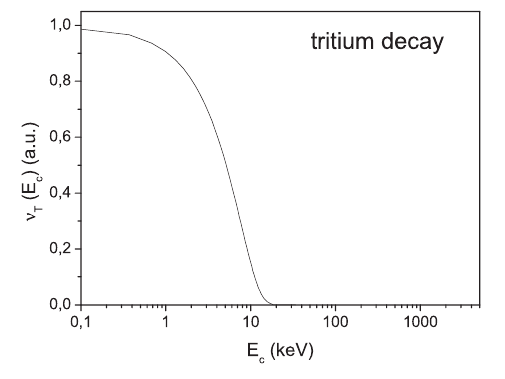
\includegraphics[width=0.95\linewidth]{solisRunawayRenerationTritium} \\ а)
    \end{minipage}
    \hfill
    \begin{minipage}[b][][b]{0.49\linewidth}\centering
        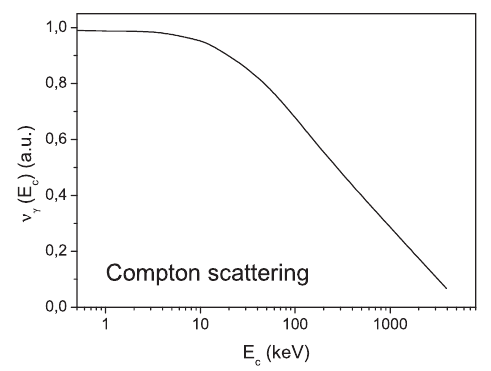
\includegraphics[width=0.95\linewidth]{solisRunawayRenerationCompton} \\ б)
    \end{minipage}
    \caption{ Зависимость скорости генерации убегающих электронов для механизма генерации из электронов, рождённых в ходе радиоактивного распада трития (а) и для механизма генерации за счёт комптоновского рассеяния (б). По вертикальной оси отложена величина $\nu \equiv (1/n_e) \cdot ( dn_r / dt ) $, нормированная на 1 при $\varepsilon_c = 0$; по горизонтальной --- критическая энергия, равная $v_c^2 m_e / 2 $ \cite{MartinSolis2017}. }
    \label{fig:solisGeneration}
\end{figure}


% ==========================================================

\subsection{Рождение электронов в токамаке}



% ==========================================================

\section{Механизмы ограничения энергии убегающих электронов}

На реальных установках существует ряд механизмов, которые ограничивают максимальную энергию убегающих электронов: 

\begin{itemize}
  \item ограничение энергии, набираемой электроном в электрическом поле токамака за время своего ускорения;
  \item синхротронное и тормозное излучение;
  \item дрейфовое смещение орбиты;
  \item взаимодействие с возмущением магнитного поля;
  \item плазменные неустойчивости.
\end{itemize}

Рассмотрим эти механизмы подробнее.

% ----------------------------------------------------------

\subsection{Ограничение энергии, набираемой электроном в электрическом поле токамака}

Ускорение убегающего электрона в плазме можно описать с помощью следующих уравнений в первом приближении \cite{MartinSolis1998,Bakhtiari2005}:
\begin{equation}
  \label{eq:AccelerationRunaways}
  \begin{alignedat}{1}
    \frac{ d p_{\parallel} }{ d t } & = e E_{\parallel} - \frac{ n_c e^4 \Lambda m_e }{ 4 \pi \epsilon_0^2 } \gamma ( Z_{eff} + 1 + \gamma ) \frac{ p_{\parallel} }{ p^3 } - ( F_s + F_b ) \frac{ p_{\parallel} }{ p }   \\
    \frac{ d p }{ d t } & = e E_{\parallel} \frac{ p_{\parallel} }{ p } - \frac{ n_c e^4 \Lambda m_e }{ 4 \pi \epsilon_0^2 } \frac{ \gamma^2 }{ p^2 } - ( F_s + F_b )
  \end{alignedat}  
\end{equation}
где $ p_{\parallel} $ --- компонента импульса, параллельная магнитному (тороидальному) полю, $p$ --- полный импульс убегающего электрона, $\gamma = 1 + p^2 / ( m_e c )^2$ --- релятивистский гамма-фактор, $Z_{eff}$ --- эффективный заряд ионов в плазме. 

Первый член правой части уравнений~\ref{eq:AccelerationRunaways} отвечает за за ускорение электронов в тороидальном электрическом поле, второй --- за торможение в результате столкновений с частицами в плазме. Последнее слагаемое, включающее в себя сумму сил $F_s + F_b$, отвечает за радиационные потери энергии за счёт синхротронного и тормозного излучения и будет рассмотрен позднее.

Если в нулевом приближении пренебречь торможением электрона и радиационными потерями, то должно быть очевидно, что за время разряда токамака с момента своего рождения электрон может набрать только конечную энергию, которая определяется временем ускорения и электрическим полем в плазме за время ускорения. Эта величина может быть грубо оценена в предположении, что $v = c$ как

\begin{equation*}
  \varepsilon(t) = \frac{ e c }{ 2 \pi R_0 } \int \limits_{t_b}^{t} V_{loop}(t') d t'
\end{equation*}
где $t_b$ --- время перехода электрона в режим убегания, $V_{loop}$ --- напряжение обхода. Очевидно, что реальная энергия электрона всегда будет меньше этой величины \cite{Shevelev2019th}.

% ----------------------------------------------------------

\subsection{Синхротронное и тормозное излучение}

В уравнениях~\ref{eq:AccelerationRunaways} присутствует сила, отвечающая за торможение убегающих электронов в результате потерь энергии на синхротронное излучение, которая равна \cite{MartinSolis1998, MartinSolis1999} 
\begin{equation*}
  F_s = \frac{2}{3} r_e m_e c^2 \left( \frac{v}{c} \right)^3 \gamma^4 \langle \frac{1}{R^2} \rangle
\end{equation*}
где $r_e = e^2/(4 \pi \epsilon_0 m_e c^2 )$ --- классический радиус электрона, $v$ --- скорость электрона, $R$ --- радиус кривизны траектории убегающего электрона. Орбита электрона в токамаке 
состоит из двух частей: движения ведущего центра вдоль силовых линий магнитного поля и ларморовского вращения. В приближении, что большой радиус токамака $R_0$ намного больше, чем ларморовский радиус $r_g$, можно написать выражение для среднего радиуса кривизны траектории убегающего электрона \cite{MartinSolis1998}:
\begin{equation*}
  \langle \frac{1}{R^2} \rangle \approx \frac{1}{R_0^2} + \frac{ \sin(\theta)^4 }{r_g^2}
\end{equation*}
где $\theta$ --- пинч-угол. 

На рис.~\ref{fig:solisRunawayPhaseDiagram} показана фазовая диаграмма решения системы уравнений~\ref{eq:AccelerationRunaways}. Для каждого значения электрического поля существуют два значения $p_{\parallel}$ и $p_{\perp}$, соответствующие двум особым точкам $P_1$ и $P_2$. Эти две особые точки имеют вполне определенный физический смысл: ветвь седловой точки $P_1$ дает критическую энергию для генерации убегающих электронов, а устойчивый фокус в точке $P_2$ даёт энергетический предел для генерируемых убегающих электронов.

\begin{figure}[ht]
  \centerfloat{ 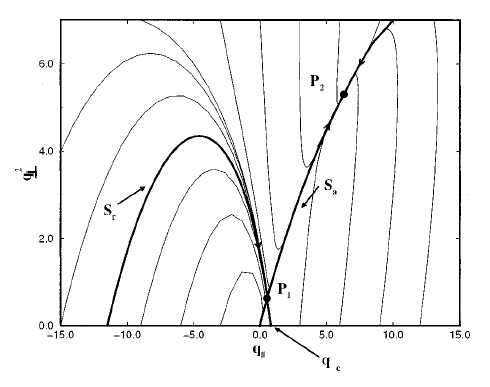
\includegraphics[width=0.60\linewidth]{solisRunawayPhaseDiagram} }
  \caption{ Фазовая диаграмма решения системы уравнений~\ref{eq:AccelerationRunaways} в координатах $q_{\parallel} = p_{\parallel}/(m_e c)$ и $q_{\perp} = p_{\perp}/(m_e c)$ для параметров ( $E_{\parallel} m_e c^2 )/(T_e E_D ) = 4.4$, $ 1 + Z_{eff} = 4 $, $ 2 \epsilon_0 B_0^2 / 3 n_e = 0.65 $, $ ( m_e c / e B_0 R_0 )^2 \cdot 2 \epsilon_0 B_0^2 / 3 n_e = 2.3 \cdot 10^{-8} $, $F_b = 0$ ~\cite{MartinSolis1998}.}
  \label{fig:solisRunawayPhaseDiagram}
\end{figure}

Предельными траекториями частиц, проходящих через точки $P_1$ и $P_2$, являются сепаратрисы $S_r$ и $S_a$. Сепаратриса $S_r$ делит фазовое пространство на две области, причем область вне $S_r$ составляет область убегания: все электроны, первоначально находившиеся вне $S_r$, в конце концов будут двигаться вдоль $S_a$ к устойчивому фокусу $P_2$. Электроны, изначально находившиеся внутри $S_r$, будут двигаться в начало координат, т.е. они не переходят в режим убегания. Устойчивая точка $P_2$ является следствием учёта радиационных потерь в уравнениях. Убегающие электроны не непрерывно ускоряются тороидальным электрическим полем, вместо этого они достигают максимальной энергии, когда мощность, излучаемая электроном, равна получению энергии от электрического поля.  

Сила, действующая на убегающий электрон вследствие потерь энергии на тормозное излучение, может быть записана для однокомпонентной плазмы как \cite{Bakhtiari2005}
\begin{equation*}
  F_b = \frac{4}{137} n_e ( Z_{eff} + 1 ) m_e c^2 \gamma r_e^2 \left( \ln 2 \gamma - \frac{1}{3} \right)
\end{equation*}

Отметим, что синхротронное излучение зависит от тороидального магнитного поля, большого радиуса токамака и скорости электронов, а сила, действующая на электрон из-за тормозного излучения, не зависит от магнитного поля и большого радиуса, но зависит от концентрации и эффективного заряда $Z_{eff}$ в плазме. При нормальной работе термоядерного токамака $Z_{eff}$ имеет низкое значение, чуть выше единицы, но в случае чрезвычайной ситуации, когда токамак необходимо быстро отключить, может быть введено огромное количество примесей с высоким $Z$, повышая тем самым $Z_{eff}$. 

% ----------------------------------------------------------

\subsection{Дрейфовое смещение орбиты}

С ростом энергии электрона траектория убегающего электрона будет смещаться в сторону слабого магнитного поля токамака. В некоторый момент траектория электрона пересекается с лимиттером или с первой стенкой токамака, в результате чего электрон гибнет \cite{MartinSolis1999,Carbajal2017}. В предположении плоского профиля тока по плазме это происходит при энергии \cite{Knoepfel1979,MartinSolis1999}

\begin{equation*}
  \gamma = \left[ \left( 2 R_0 ( 1 - r_c / r_l ) \frac{I_p}{17000} \right)^2 + 1 \right]^{\frac{1}{2}}
\end{equation*}
где $r_c$ --- малый радиус, на котором электрон перешёл в режим убегания, $r_l$ --- радиус, на котором расположен лимиттер или первая стенка, $I_p$ --- ток по плазме. Пример расчётных орбит показан на рис.~\ref{fig:breizmanOrbits}

\begin{figure}[ht]
  \centerfloat{ 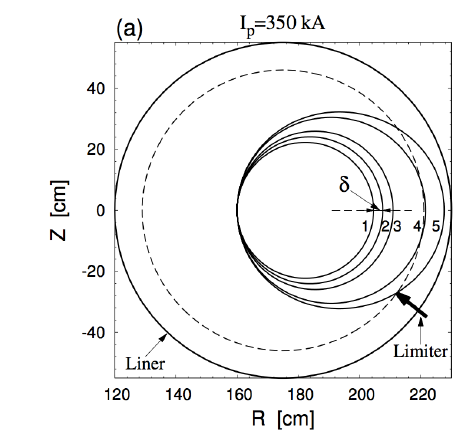
\includegraphics[width=0.60\linewidth]{breizmanOrbits} }
  \caption{ Траектории ведущих центров убегающих электронов при различных значениях энергии. Токамак TEXTOR, $I_p = 350$~кА, $B_0 = 2.5$~Т, кривые 1--5 соответствуют энергиям 10~кэВ, 10~МэВ, 20~МэВ, 40~МэВ, 46~МэВ\cite{Breizman2019,Abdullaev2016}.}
  \label{fig:breizmanOrbits}
\end{figure}

% ----------------------------------------------------------

\subsection{Взаимодействие с возмущениями магнитного поля}

Магнитное поле токамака является неоднородным из-за конечного числа обмоток. Резонанс между движением электронов по ларморовской окружности и гармониками пульсации тороидального поля, возникающими вследствие конечного числа обмоток, увеличивает компоненту скорости, перпендикулярную направлению магнитного полю \cite{MartinSolis1998,MartinSolis1999,Laurent1990}. Взаимодействие с n-й гармоникой пульсаций тороидального поля происходит при энергии электрона 
\begin{equation*}
  \gamma_n \approx \frac{ e B_0 R_0 }{ n N_c m_e c }
\end{equation*}
где $N_c$ --- число катушек тороидального поля, $n$ --- номер тороидальной гармоники. Эффективность механизма пульсаций для ограничения энергии убегающих электронов сильно зависит от амплитуды пульсаций: при заданном электрическом поле для эффективного взаимодействия необходима достаточно большая амплитуда пульсаций. В токамаке сила пульсаций больше для низких номеров тороидальных гармоник и быстро затухает по радиусу от края плазмы. Поэтому следует ожидать, что эффекты будет наиболее существенным в периферийных областях плазмы \cite{MartinSolis1998}.

%и при малых значениях числа тороидальной гармоники. Экспериментальные доказательства эффективного взаимодействия убегания и пульсаций были получены в нескольких устройствах [9, 12, 13], и было предсказано, что резонанс между электронной гирочастотой и основной частотой пульсаций может создать верхнюю границу энергии убегания во время разрушения плазмы в большие токамаки, такие как Joint European Torus ~JET!14 или 15ITER. Анализ динамики взаимодействия между пульсациями тороидального поля и убегающим движением с использованием представленного здесь описания пробных частиц уже рассматривался в предыдущей работе16 и станет предметом будущей публикации.

% ----------------------------------------------------------

\subsection{Плазменные неустойчивости}

На существование убегающих электронов в плазме так же оказывают влияние различные неустойчивости. 

Стоит особо отметить веерную неустойчивость. Как правило, эта неустойчивость развивается в разрядах с невысокой плотностью (менее $10^{19}$~м${}^{-3}$. Неустойчивость проявляется в виде коротких (10--100~мкс) периодических всплесков увеличения диамагнетизма плазмы; время между соседними всплесками намного превышает продолжительность каждого из них (1--2~мс).  Одновременно с измене- изменением диамагнетизма наблюдается резкое увеличение интенсивности рентгеновского и синхротронного излучения плазмы, меняется напряжение на обходе плазменного шнура. Развитие этой неустойчивости может ограничивать энергию убегающих электронов и приводить к аномальной диффузии к стенке токамака. \cite{Parail1978,Leontovich1982}

Существенно влияние различных МГД неустойчивостей, которые приводят к выходу убегающих электронов, существующих в плазме, на переферию плазмы, а электроны с периферии выходят на стенки или лимиттер токамака. Соответствующие всплески рентгеновского излучения неоднократно наблюдались на небольших установках \cite{Shevelev2016,Shevelev2018}. 


% ==========================================================

\section{Методы диагностики убегающих электронов}\label{sec:ch1/sec2}

Ы!

% ==========================================================

\FloatBarrier
